\documentclass[bachelor, och, referat]{SCWorks}
\usepackage[T2A]{fontenc}
\usepackage[utf8]{inputenc}
\usepackage{graphicx}
\usepackage{pgfplots}
\pgfplotsset{compat=1.9}
\usepackage[dvips]{graphicx}
\usepackage{amsmath}
\usepackage{amssymb}
\usepackage{amsthm}
\usepackage{fancyvrb}
\usepackage{longtable}
\usepackage{array}
\usepackage[english,russian]{babel}
\usepackage{minted}
\usepackage{tempora}
\usepackage[colorlinks=false]{hyperref}
\hypersetup{
colorlinks,
citecolor=black,
filecolor=black,
linkcolor=black,
urlcolor=black
}
\AtBeginEnvironment{minted}{\renewcommand{\fcolorbox}[4][]{#4}}

\newcommand{\eqdef}{\stackrel {\rm def}{=}}
\newtheorem{lem}{Лемма}

\begin{document}
\chair{математической кибернетики и компьютерных наук}
\title{Параллельное и распределенное программирование. Work06}
\course{3}
\group{311}
\napravlenie{02.03.02 "--- Фундаментальная информатика и информационные технологии}
\studenttitle{студента}
\author{Вильцева Данила Денисовича}

\satitle{Старший преподаватель}
\saname{М.\,С.\,Портенко}

\term{6}
\date{2023}

\maketitle
\tableofcontents


%---------------------------------------------------------------------------------------------

\section{Work 6}
\subsection{Условие задачи}
Выполните разработку параллельного варианта для одного из итерационных методов:

3. верхней релаксации.

Для тестовой матрицы из нулей и единиц проведите вычислительные эксперименты, результаты занесите в таблицу 1.

Таблица 1. Время выполнения последовательного и параллельного итерационного алгоритмов решения систем линейных уравнений и ускорение
\begin{figure}[h]
\center{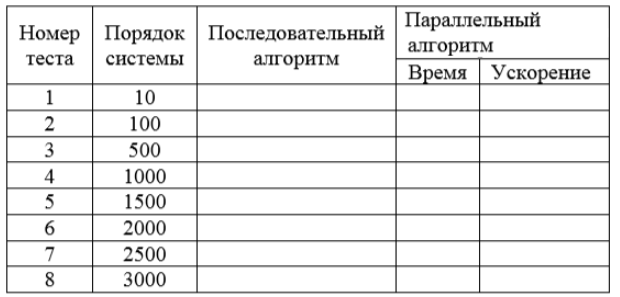
\includegraphics[scale=0.7]{task6_1.png}}
\end{figure}

Какой из алгоритмов Гаусса или итерационный обладает лучшими показателями ускорения? Заполните таблицу 2.


Таблица 2. Ускорение параллельных алгоритмов Гаусса и итерационного (вариант) решения систем линейных уравнений

\begin{figure}[h]
\center{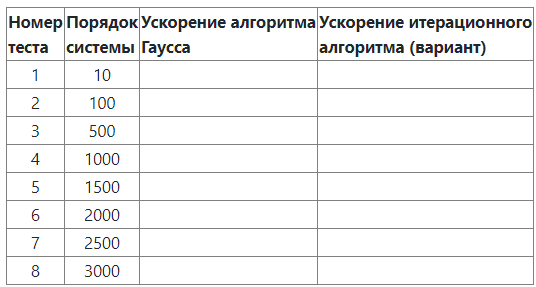
\includegraphics[scale=0.7]{task6_2.png}}
\end{figure}


\newpage

\subsection{Решение}
\textbf{Последовательная реализация метода верхней релаксации} 

\begin{figure}[h]
\center{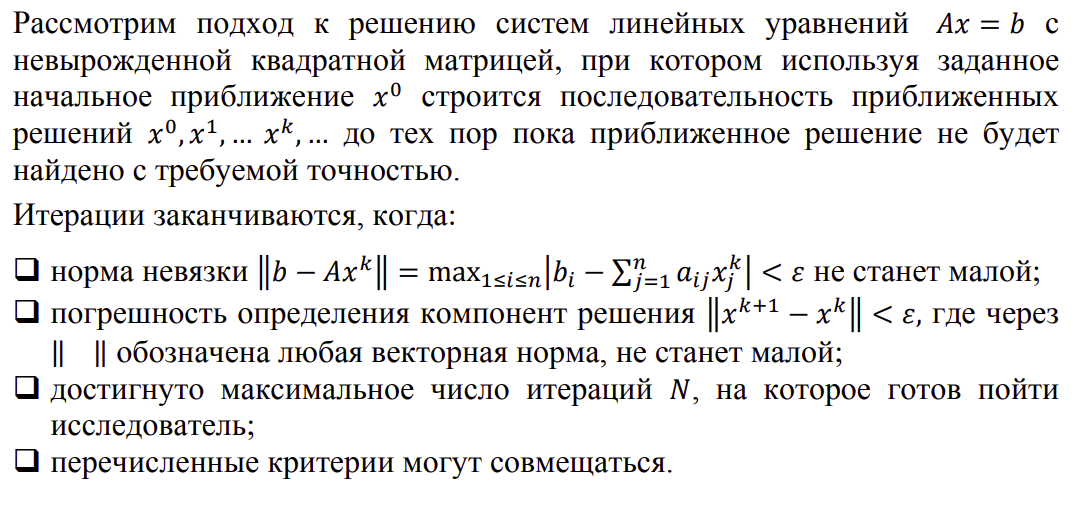
\includegraphics[scale=0.5]{task6_3.png}}
\end{figure}

\begin{figure}[h]
\center{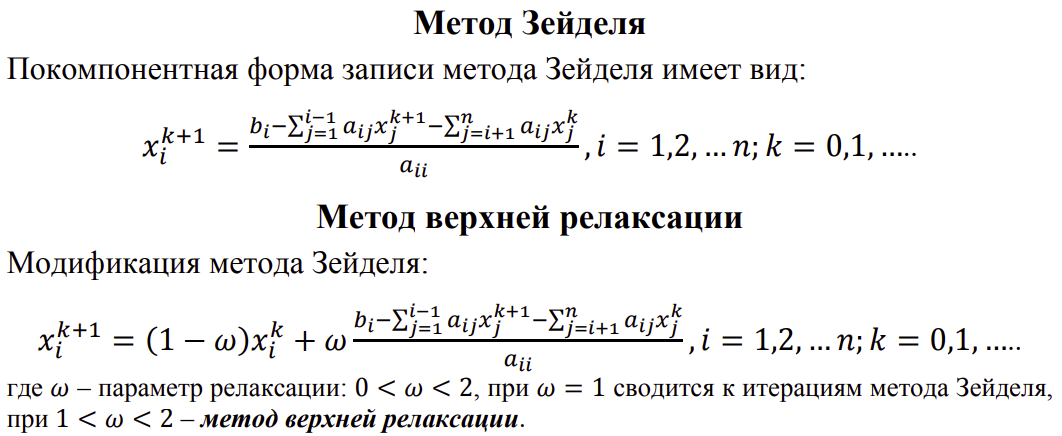
\includegraphics[scale=0.5]{task6_4.png}}
\end{figure}

\subsection{Фрагмент кода (последовательная реализация)}
\begin{minted}[breaklines, fontsize=\footnotesize]{cpp}
#include <omp.h>
#include <iostream>
#include <time.h>
#include <cmath>
#include <windows.h>
#include<cstdlib>
using namespace std;
// Function that converts numbers form LongInt type to
// double type
double LiToDouble(LARGE_INTEGER x) {
	double result = ((double)x.HighPart) * 4.294967296E9 +
		(double)((x).LowPart);
	return result;
}

// Function that gets the timestamp in seconds
double GetTime() {
	LARGE_INTEGER lpFrequency, lpPerfomanceCount;
	QueryPerformanceFrequency(&lpFrequency);
	QueryPerformanceCounter(&lpPerfomanceCount);
	return LiToDouble(lpPerfomanceCount) / LiToDouble(lpFrequency);
}

double* upper_relaxation_method(double** a, double* b, int n, double eps, double w, double* x, double* xn) {
	int i, j, k = 0;
	double norma;

	for (i = 0; i < n; i++)
	{
		xn[i] = 0;
		x[i] = xn[i];
	}
	do
	{
		k++;
		norma = 0;

		for (i = 0; i < n; i++)
		{
			x[i] = b[i];
			for (j = 0; j < n; j++)
			{
				if (i != j)
					x[i] = x[i] - a[i][j] * x[j];
			}
			x[i] /= a[i][i];

			x[i] = w * x[i] + (1 - w) * xn[i];

			if (fabs(x[i] - xn[i]) > norma)
				norma = fabs(x[i] - xn[i]);
			xn[i] = x[i];
		}
	} while (norma > eps);

	return x;

}

double experiment(double* res, double** a, double* b, int n, double eps, double w, double* x, double* xn)
{
	double stime, ftime; // время начала и конца расчета
	stime = GetTime();
	upper_relaxation_method(a, b, n, eps, w, x, xn); // вызов функции интегрирования
	ftime = GetTime();
	return (ftime - stime) / CLOCKS_PER_SEC;
}


int main()
{
	setlocale(LC_CTYPE, "RUSSIAN");
	int n;
	double eps;
	double w;

	cout << "Введите размерность матрицы N*N:";
	cin >> n;
	double** a = new double* [n];
	for (int i = 0; i < n; i++)
		a[i] = new double[n];


	double* b = new double[n];
	double* x = new double[n];
	double* xn = new double[n];

	for (int i = 0; i < n; i++)
	{
		for (int j = 0; j < n; j++)
		{

			a[i][j] = rand() / double(1000);
		}
	}

	for (int i = 0; i < n; i++)
	{

		b[i] = rand() / double(1000);
	}

	eps = 0.001;
	w = 1.12;

	double time; // время проведенного эксперимента
	double res; // значение вычисленного интеграла
	double min_time; // минимальное время работы
					 // реализации алгоритма
	double max_time; // максимальное время работы
					 // реализации алгоритма
	double avg_time; // среднее время работы
					 // реализации алгоритма
	int numbExp = 10; // количество запусков программы

	// первый запуск
	min_time = max_time = avg_time = experiment(&res, a, b, n, eps, w, x, xn);
	// оставшиеся запуски
	for (int i = 0; i < numbExp - 1; i++)
	{
		time = experiment(&res, a, b, n, eps, w, x, xn);
		avg_time += time;
		if (max_time < time) max_time = time;
		if (min_time > time) min_time = time;
	}
	// вывод результатов эксперимента
	cout << "execution time : " << avg_time / numbExp << "; " <<
		min_time << "; " << max_time << endl;
	cout.precision(8);
}
\end{minted}

\textbf{Параллельная реализация метода верхней релаксации} 

Используем директиву #pragma omp parallel for, которая создаст несколько вычислительных потоков и разделит итерации между ними.

\subsection{Фрагмент кода (параллельная реализация)}
\begin{minted}[breaklines, fontsize=\footnotesize]{cpp}
#include <omp.h>
#include <iostream>
#include <time.h>
#include <cmath>
#include <windows.h>
#include<cstdlib>
using namespace std;
// Function that converts numbers form LongInt type to
// double type
double LiToDouble(LARGE_INTEGER x) {
	double result = ((double)x.HighPart) * 4.294967296E9 +
		(double)((x).LowPart);
	return result;
}

// Function that gets the timestamp in seconds
double GetTime() {
	LARGE_INTEGER lpFrequency, lpPerfomanceCount;
	QueryPerformanceFrequency(&lpFrequency);
	QueryPerformanceCounter(&lpPerfomanceCount);
	return LiToDouble(lpPerfomanceCount) / LiToDouble(lpFrequency);
}

double* upper_relaxation_method(double** a, double* b, int n, double eps, double w, double* x, double* xn) {
	int i, j, k = 0;
	double norma;
#pragma omp parallel for
	for (i = 0; i < n; i++)
	{
		xn[i] = 0;
		x[i] = xn[i];
	}
	do
	{
		k++;
		norma = 0;

		for (i = 0; i < n; i++)
		{
			x[i] = b[i];
#pragma omp parallel for
			for (j = 0; j < n; j++)
			{
				if (i != j)
					x[i] = x[i] - a[i][j] * x[j];
			}
			x[i] /= a[i][i];

			x[i] = w * x[i] + (1 - w) * xn[i];

			if (fabs(x[i] - xn[i]) > norma)
				norma = fabs(x[i] - xn[i]);
			xn[i] = x[i];
		}
	} while (norma > eps);

	return x;

}

double experiment(double* res, double** a, double* b, int n, double eps, double w, double* x, double* xn)
{
	double stime, ftime; // время начала и конца расчета
	stime = GetTime();
	upper_relaxation_method(a, b, n, eps, w, x, xn); // вызов функции интегрирования
	ftime = GetTime();
	return (ftime - stime) / CLOCKS_PER_SEC;
}


int main()
{
	setlocale(LC_CTYPE, "RUSSIAN");
	int n;
	double eps;
	double w;

	cout << "Введите размерность матрицы N*N:";
	cin >> n;
	double** a = new double* [n];
	for (int i = 0; i < n; i++)
		a[i] = new double[n];


	double* b = new double[n];
	double* x = new double[n];
	double* xn = new double[n];

	for (int i = 0; i < n; i++)
	{
		for (int j = 0; j < n; j++)
		{

			a[i][j] = rand() / double(1000);
		}
	}

	for (int i = 0; i < n; i++)
	{

		b[i] = rand() / double(1000);
	}

	eps = 0.001;
	w = 1.12;

	double time; // время проведенного эксперимента
	double res; // значение вычисленного интеграла
	double min_time; // минимальное время работы
					 // реализации алгоритма
	double max_time; // максимальное время работы
					 // реализации алгоритма
	double avg_time; // среднее время работы
					 // реализации алгоритма
	int numbExp = 10; // количество запусков программы

	// первый запуск
	min_time = max_time = avg_time = experiment(&res, a, b, n, eps, w, x, xn);
	// оставшиеся запуски
	for (int i = 0; i < numbExp - 1; i++)
	{
		time = experiment(&res, a, b, n, eps, w, x, xn);
		avg_time += time;
		if (max_time < time) max_time = time;
		if (min_time > time) min_time = time;
	}
	// вывод результатов эксперимента
	cout << "execution time : " << avg_time / numbExp << "; " <<
		min_time << "; " << max_time << endl;
	cout.precision(8);
}
\end{minted}




\newpage
\subsection{Результат работы программы}

\textbf{Последовательная реализация метода верхней релаксации}
\begin{figure}[h]
\center{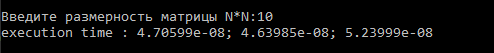
\includegraphics[scale=1.0]{task6_posl_10.png}}
\end{figure}

\begin{figure}[h]
\center{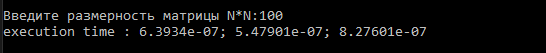
\includegraphics[scale=1.0]{task6_posl_100.png}}
\end{figure}

\begin{figure}[h]
\center{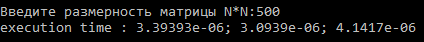
\includegraphics[scale=1.0]{task6_posl_500.png}}
\end{figure}

\begin{figure}[h]
\center{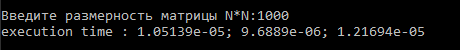
\includegraphics[scale=1.0]{task6_posl_1000.png}}
\end{figure}

\begin{figure}[h]
\center{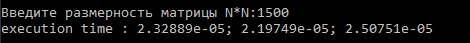
\includegraphics[scale=1.0]{task6_posl_1500.png}}
\end{figure}

\newpage

\begin{figure}[h]
\center{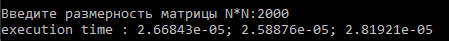
\includegraphics[scale=1.0]{task6_posl_2000.png}}
\end{figure}

\begin{figure}[h]
\center{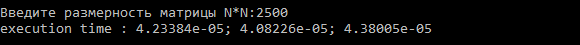
\includegraphics[scale=1.0]{task6_posl_2500.png}}
\end{figure}

\begin{figure}[h]
\center{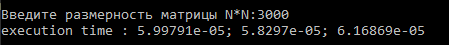
\includegraphics[scale=1.0]{task6_posl_3000.png}}
\end{figure}




\newpage
\textbf{Параллельная реализация метода верхней релаксации} 

\begin{figure}[h]
\center{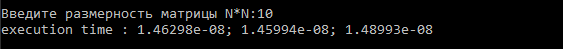
\includegraphics[scale=1.0]{task6_paral_10.png}}
\end{figure}

\begin{figure}[h]
\center{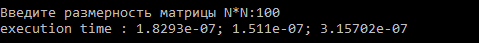
\includegraphics[scale=1.0]{task6_paral_100.png}}
\end{figure}

\begin{figure}[h]
\center{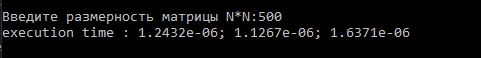
\includegraphics[scale=1.0]{task6_paral_500.png}}
\end{figure}

\begin{figure}[h]
\center{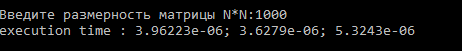
\includegraphics[scale=1.0]{task6_paral_1000.png}}
\end{figure}

\begin{figure}[h]
\center{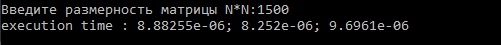
\includegraphics[scale=1.0]{task6_paral_1500.png}}
\end{figure}


\begin{figure}[h]
\center{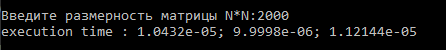
\includegraphics[scale=1.0]{task6_paral_2000.png}}
\end{figure}

\begin{figure}[h]
\center{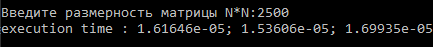
\includegraphics[scale=1.0]{task6_paral_2500.png}}
\end{figure}

\begin{figure}[h]
\center{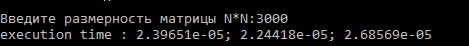
\includegraphics[scale=1.0]{task6_paral_3000.png}}
\end{figure}

\newpage
\section{Вывод}

\begin{figure}[h]
\center{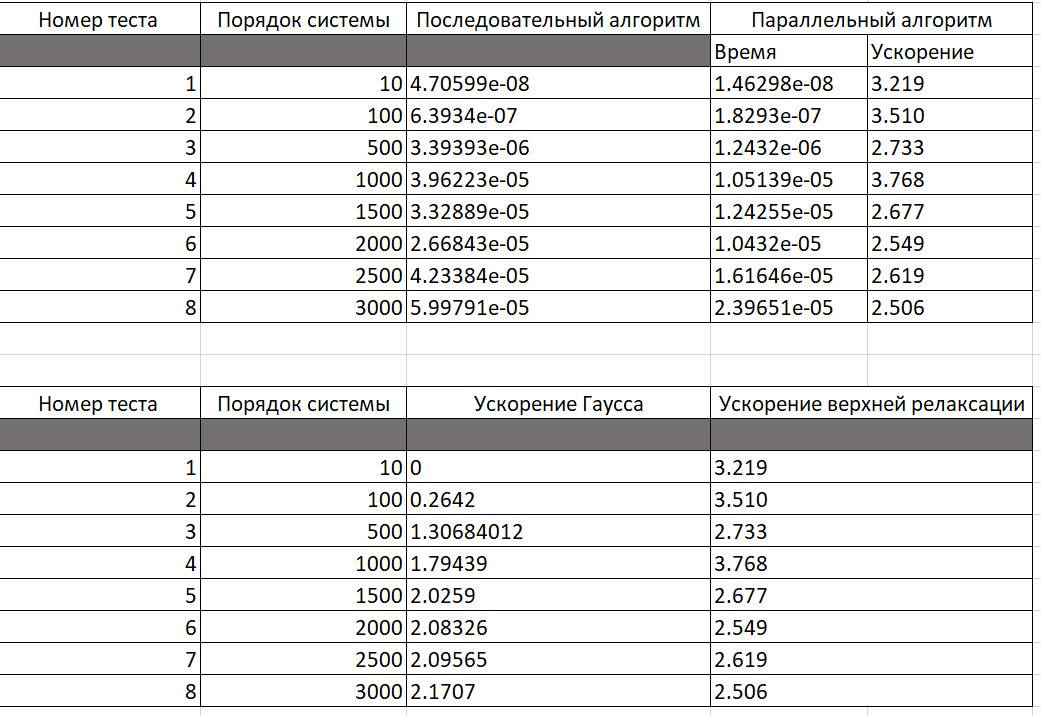
\includegraphics[scale=0.5]{task6_table.png}}
\end{figure}

Метод верхней релаксации имеет преимущество перед методом Гаусса, что видно по значениям таблицы.



\section{Характеристики компьютера}
\begin{figure}[h]
\center{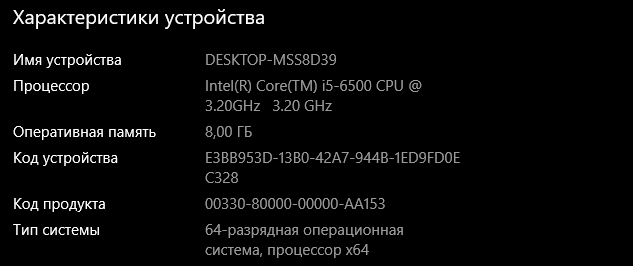
\includegraphics[scale=0.5]{system.png}}
\end{figure}
\begin{figure}[h]
\center{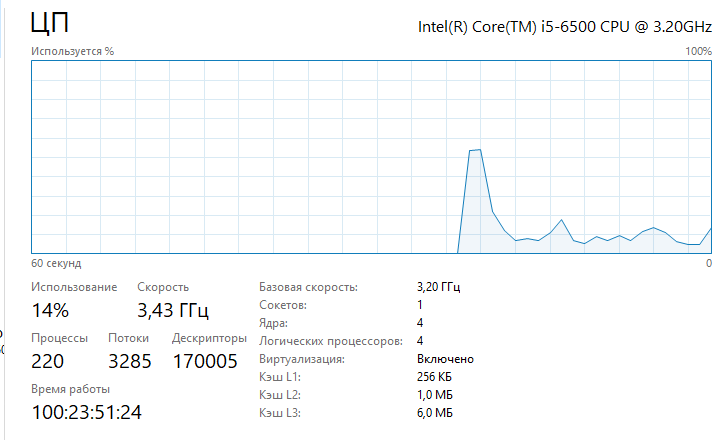
\includegraphics[scale=0.5]{system2.png}}
\end{figure}

%---------------------------------------------------------------------------------------------
\end{document}


